%% RT-plots.tex

\begin{figure}
    \centering
    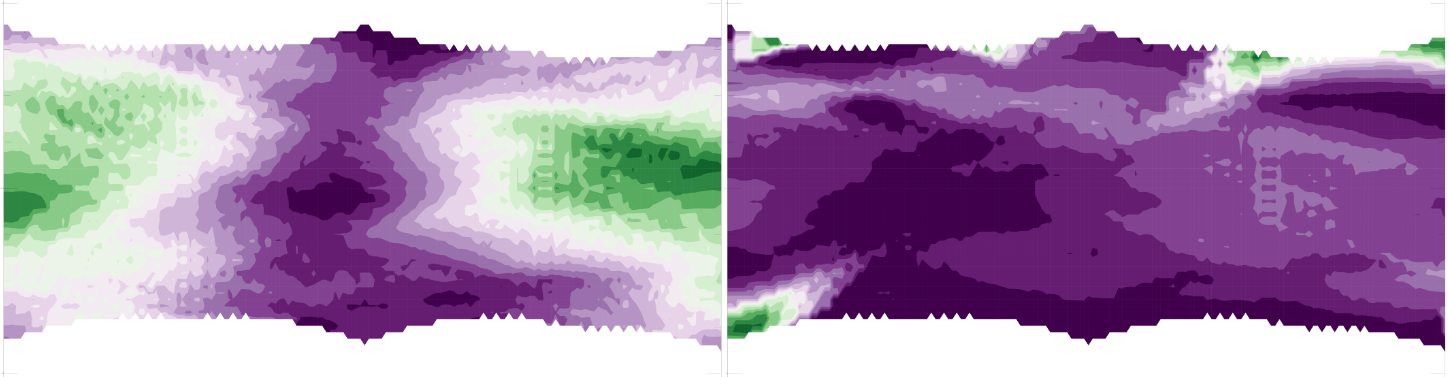
\includegraphics[width=\columnwidth]{images/RadonPlots/RT-snips/CPSB-8313-6101-RT-snip.png}
    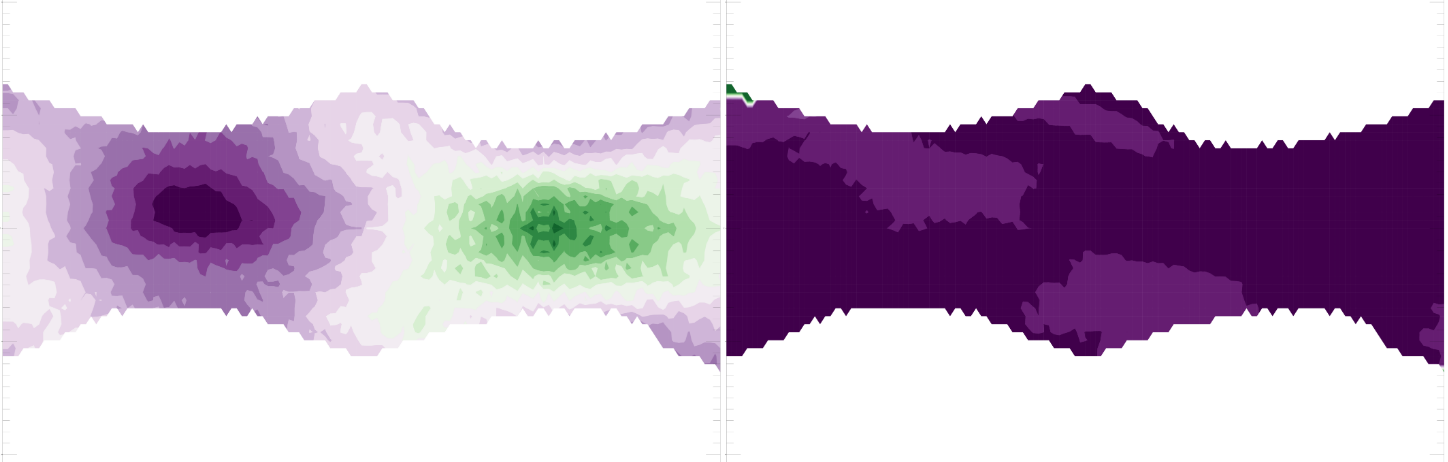
\includegraphics[width=\columnwidth]{images/RadonPlots/RT-snips/CPSB-9494-3701-RT-snip.png}
    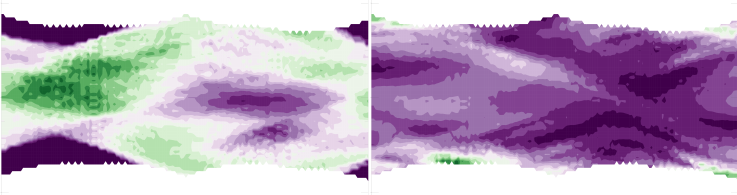
\includegraphics[width=\columnwidth]{images/RadonPlots/RT-snips/CPSB-8398-6102-RT-snip.png}
    \caption{CPSBs: Radon transforms of stellar velocity field (left) and gas velocity field (right) maps. From the top CPSB-8313-6101, CPSB-9404-3710 and CPSB -8398-6103}
    \label{fig:CPSB-RTs}
\end{figure}

\begin{figure}
    \centering
    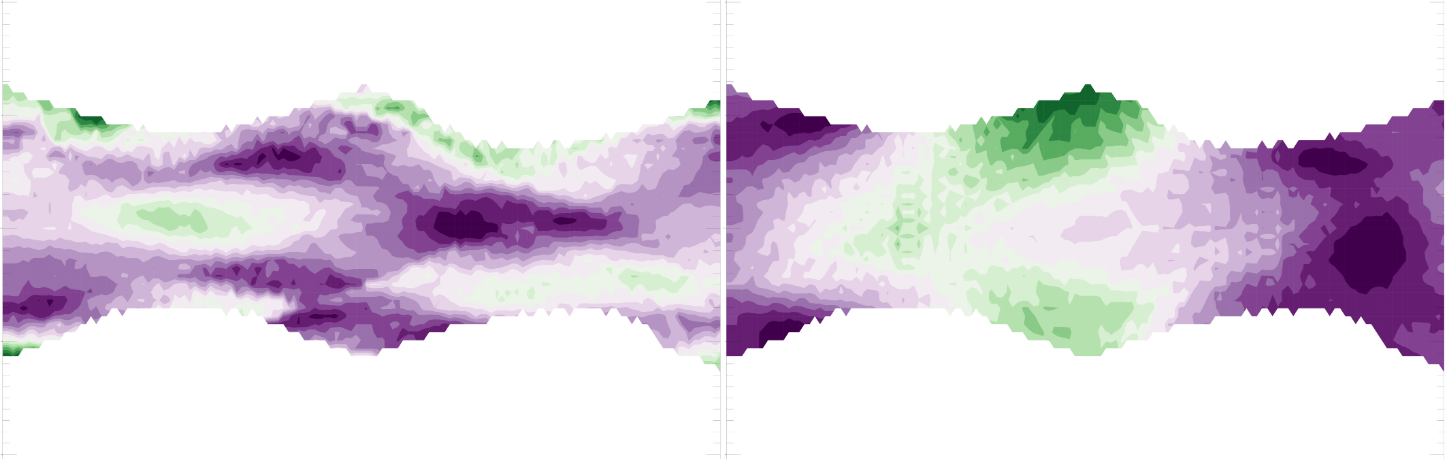
\includegraphics[width=\columnwidth]{images/RadonPlots/RT-snips/RPSB-9872-3701-RT-snip.png}
    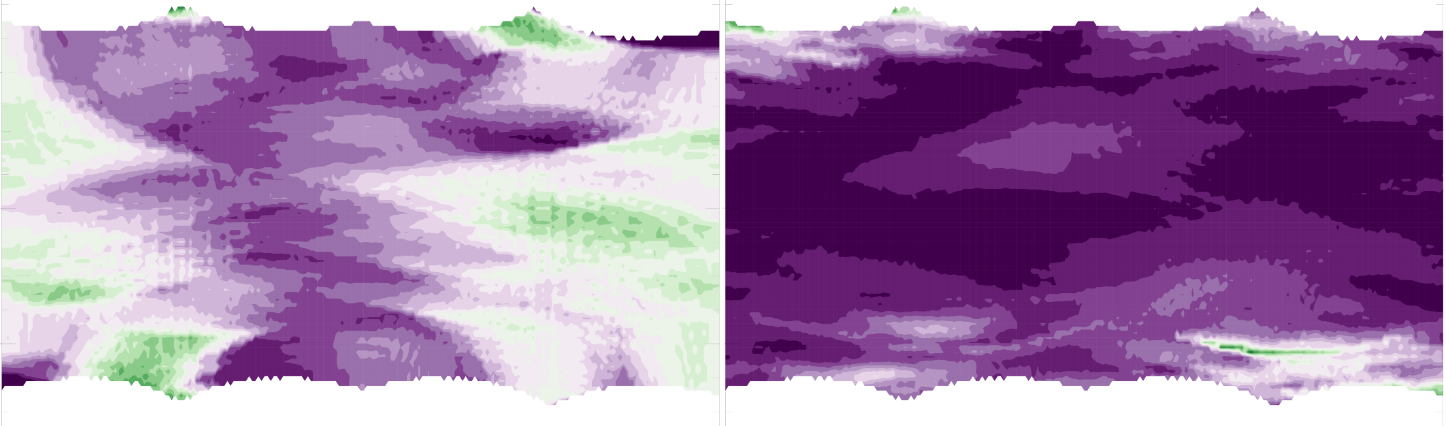
\includegraphics[width=\columnwidth]{images/RadonPlots/RT-snips/RPSB-8932-12704-RT-snip.png}
    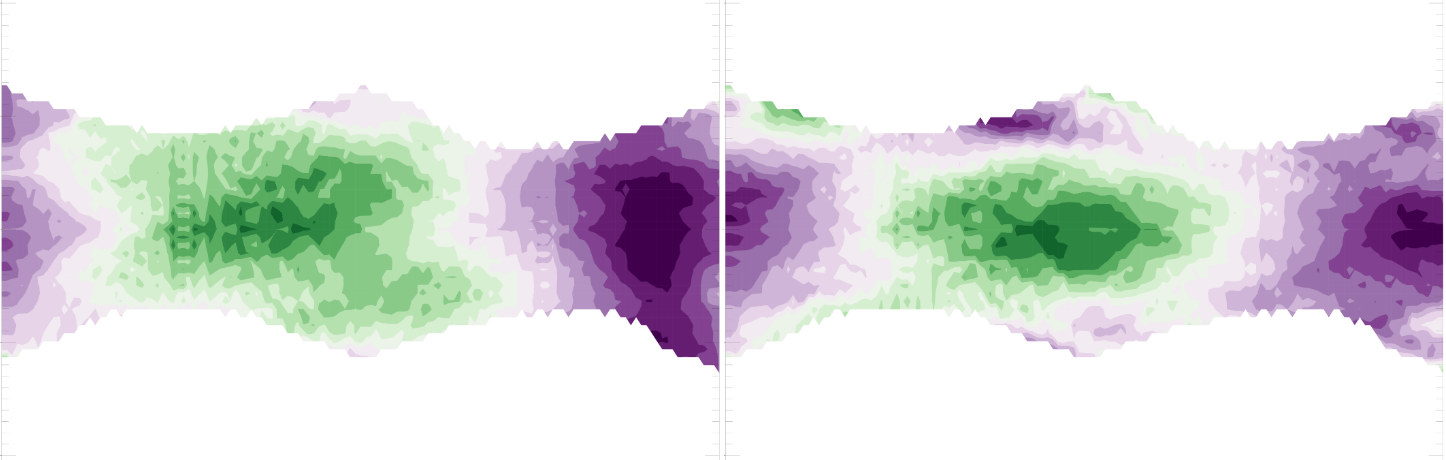
\includegraphics[width=\columnwidth]{images/RadonPlots/RT-snips/RPSB-8554-3701-RT-snip.png}
    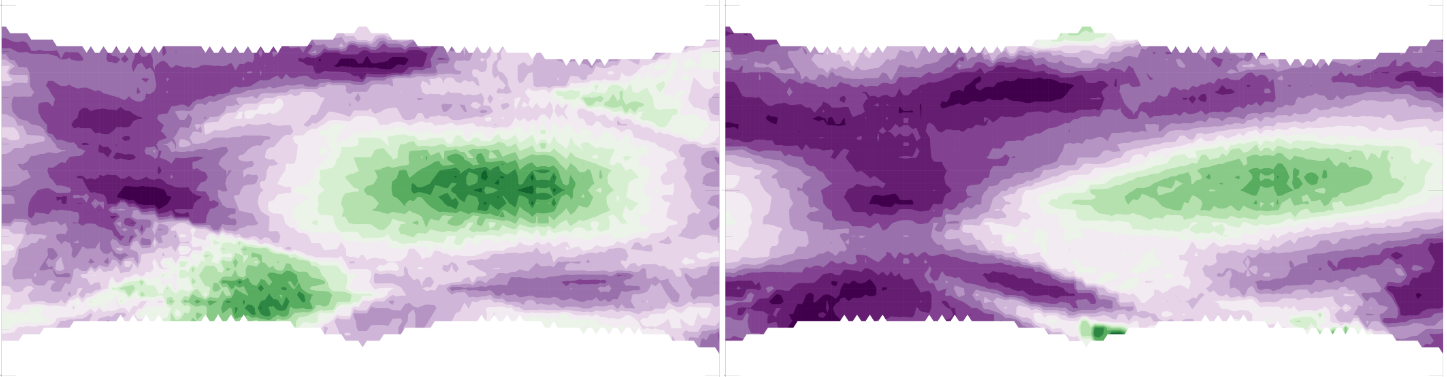
\includegraphics[width=\columnwidth]{images/RadonPlots/RT-snips/RPSB-8323-6103-RT-snip.png}
    \caption{RPSBs: layout is as per Figure \ref{fig:CPSB-RTs}, showing the Radon transform maps from the top for for RPSB-9872-3701, RPSB-8932-12704, RPSB-8554-3701 and RPSB-8323-6103.}
    \label{fig:RPSB-RTs}
\end{figure}

\begin{figure}
    \centering
    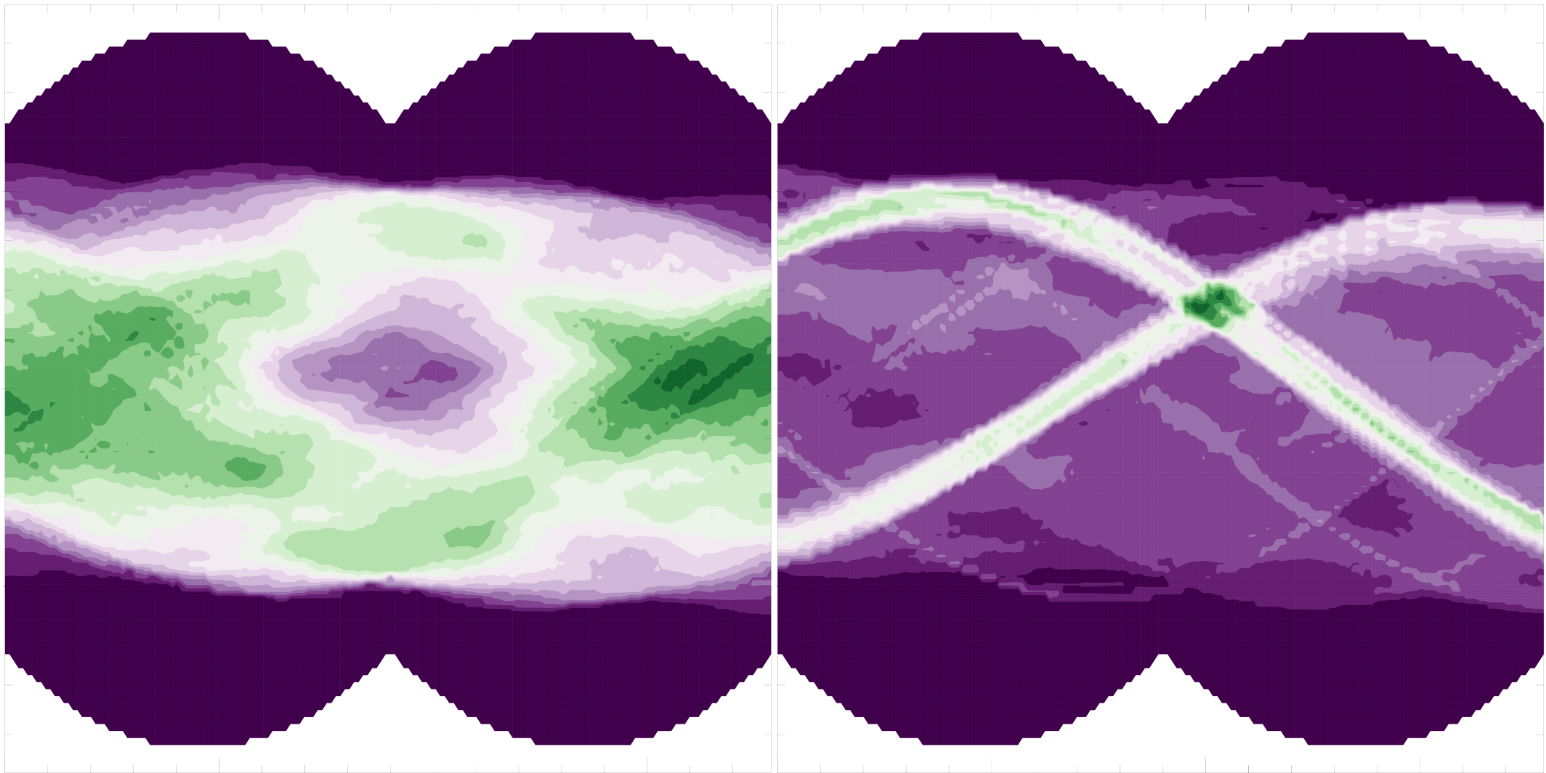
\includegraphics[width=\columnwidth]{images/RadonPlots/RT-snips/CPSB-8313-6101-SG-AP-00.png}
    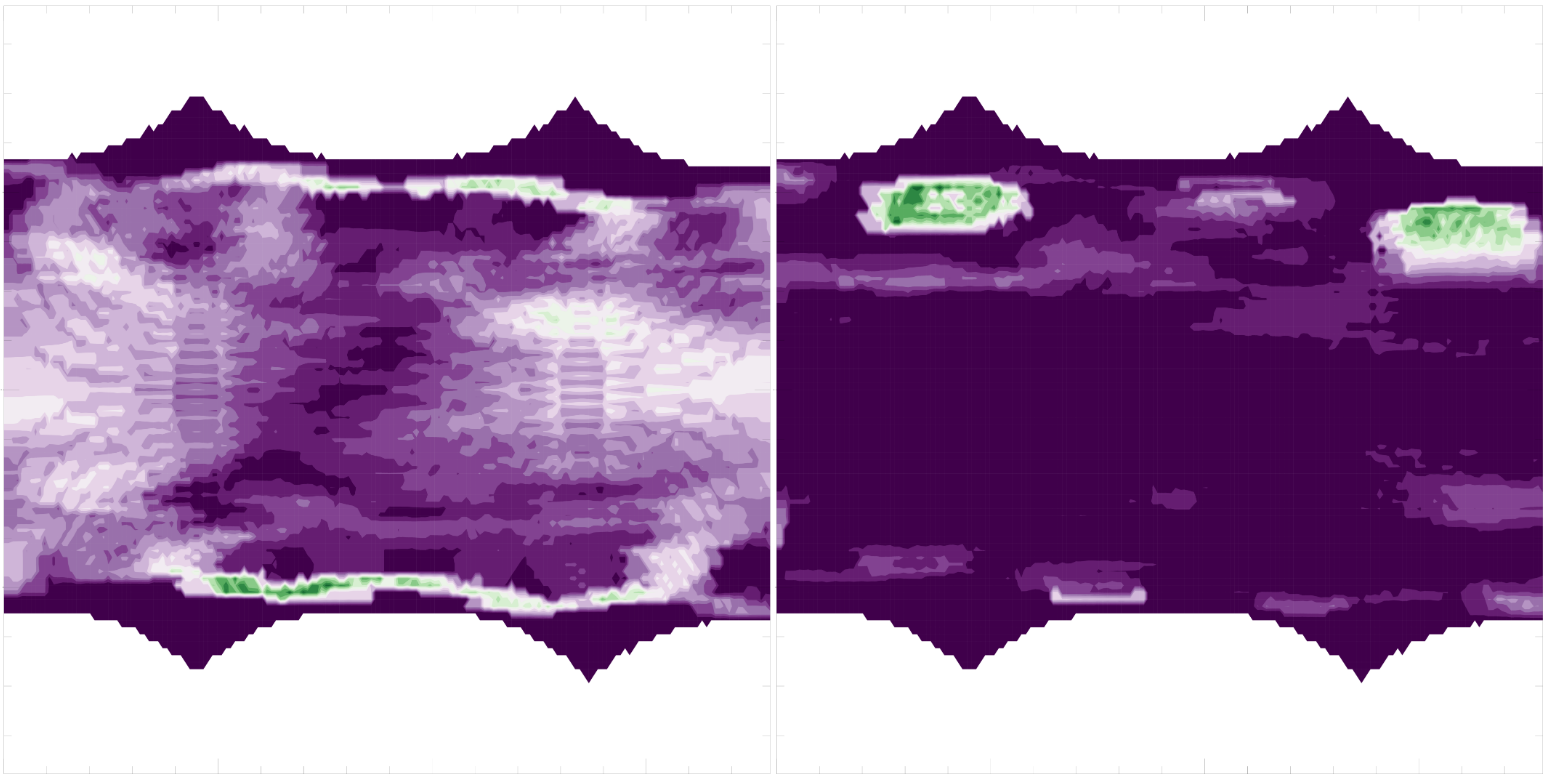
\includegraphics[width=\columnwidth]{images/RadonPlots/RT-snips/CPSB-8313-6101-SG-AP-04.png}
    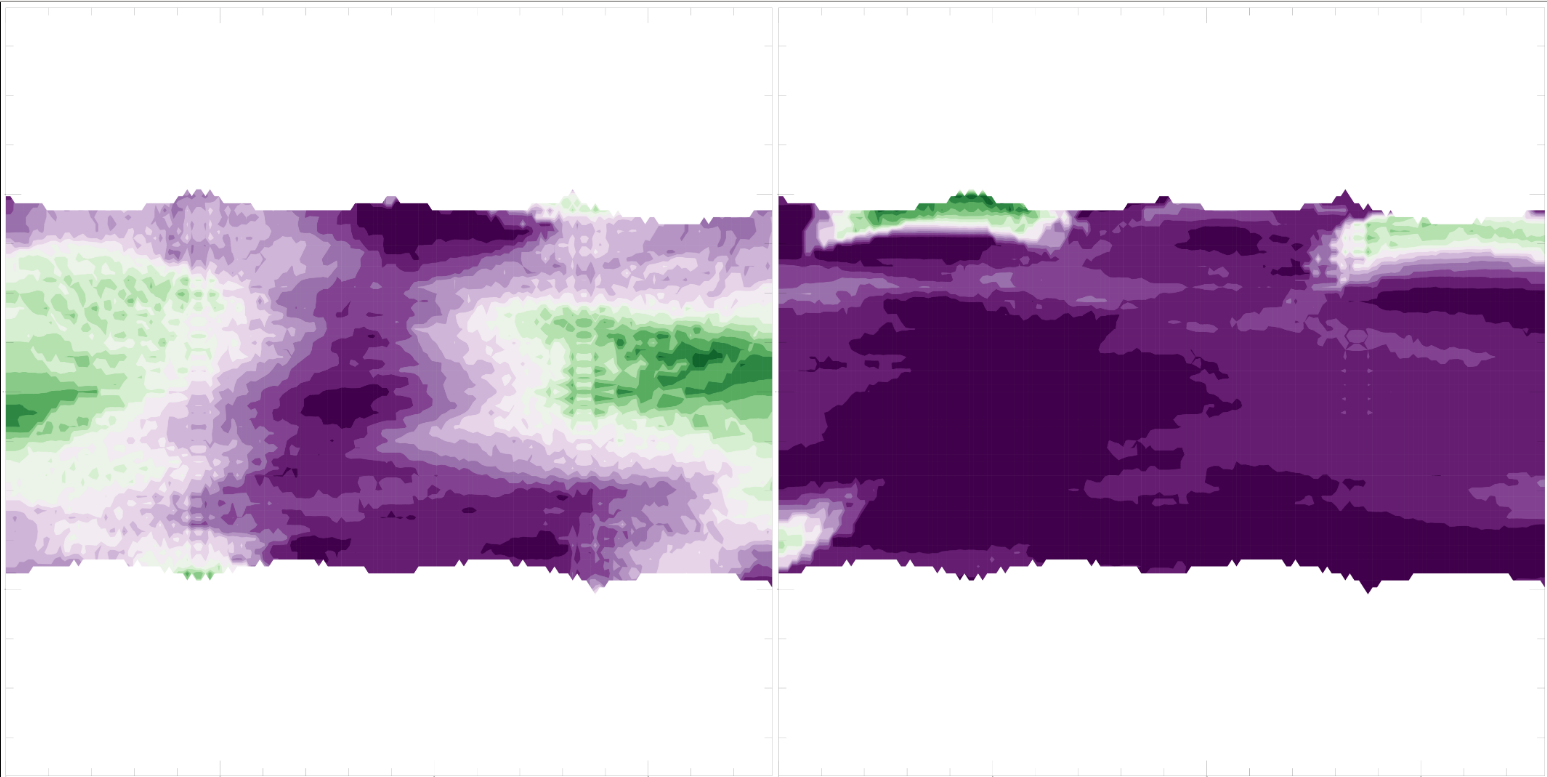
\includegraphics[width=\columnwidth]{images/RadonPlots/RT-snips/CPSB-8313-6101-SG-AP-08.png}
    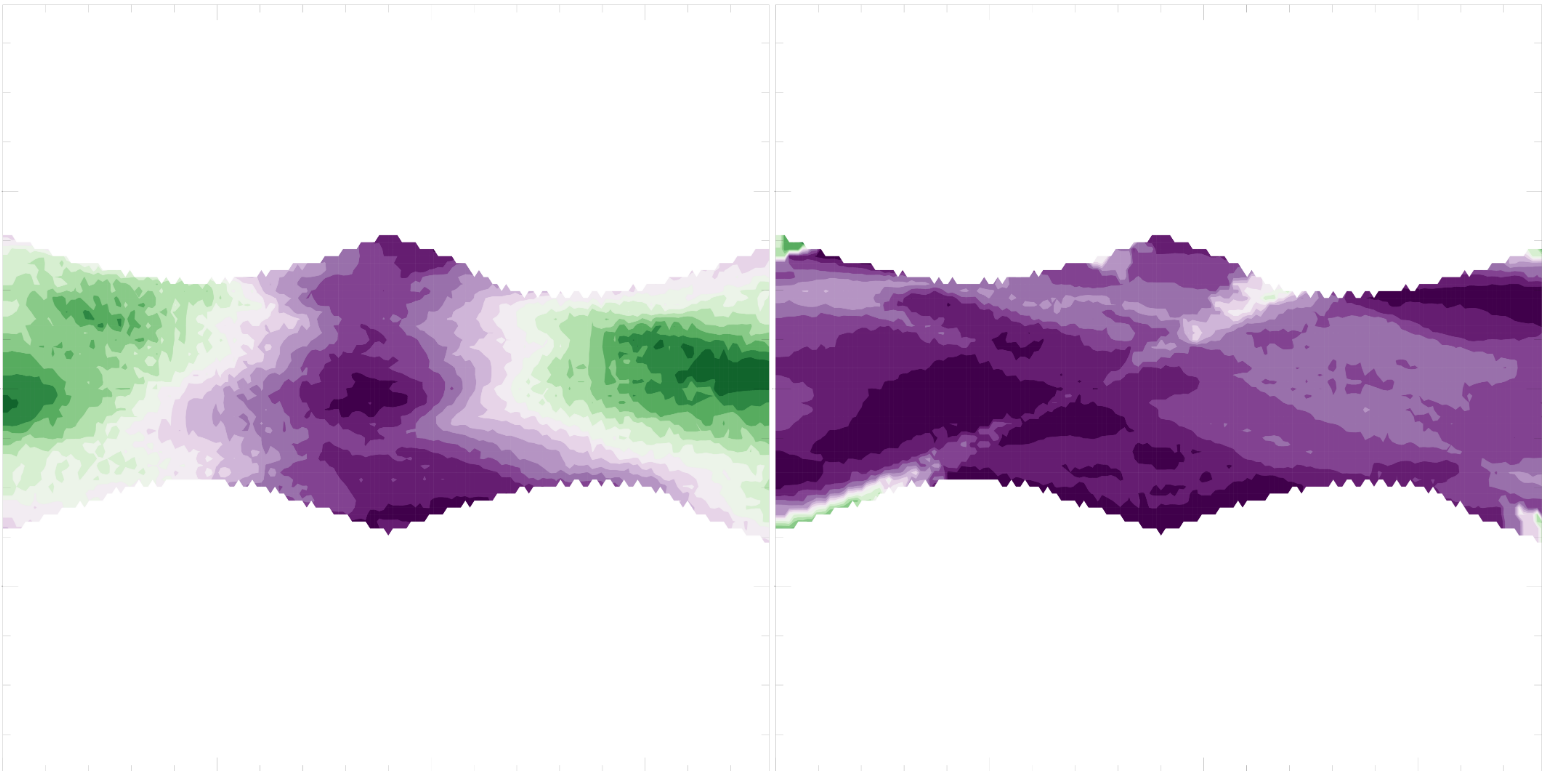
\includegraphics[width=\columnwidth]{images/RadonPlots/RT-snips/CPSB-8313-6101-SG-AP-12.png}
    \caption{CPSBs: Absolute Radon transforms of stellar velocity field (left) and gas velocity field (right) maps for CPSB-8313-6101, but with varying aperture settings. From the top $r_{ap}=0$, $r_{ap}=4$, $r_{ap}=8$ and bottom $r_{ap}=12$.}
    \label{fig:CPSB-RT-Apertures}
\end{figure}

